\section{Para que serve o decibel}
As vantagens de se representar um número qualquer em uma escala logarítmica de uma forma bem resumida são:

\begin{itemize}
    \item Números de grande valor são comprimidos;
    \item Números de baixo valor são expandidos;
    \item Permite visualizar em um mesmo gráfico grandes variações numéricas.
\end{itemize}

Para entender como essas questões podem ser interpretadas como vantagens da representação em dB, vamos tomar como exemplo a representação do ganho de um amplificador em um gráfico.

No caso de um amplificador, definimos o ganho como Av = vo/vi e podemos representar esse ganho de diferentes maneiras. Uma maneira muito comum é a representação do comportamento do ganho com a variação da frequência do sinal de entrada, um gráfico chamado de Diagrama de Resposta em Frequência ou de Diagrama de Bode (tenho ressalvas sobre o uso indiscriminado desse nome, mas vamos deixar a picuinha para outro dia). Na figura 1, mostro como é a representação do Diagrama de Resposta em Frequência do ganho de um amplificador de áudio, utilizando uma escala decimal comum.

\begin{figure}[hb]
    \centering
    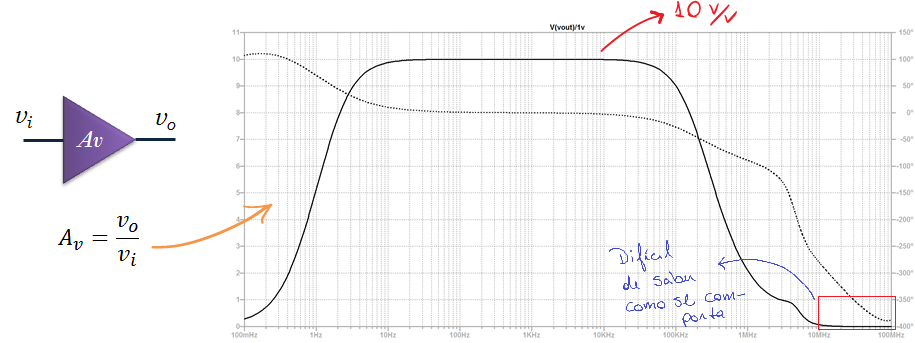
\includegraphics[width=0.45\textwidth]{imgs/diagramaderesposta.png}
    \caption{Diagrama de Resposta em Frequência de um Ganho em base decimal.}
    \label{fig:cco}
\end{figure}

É notável que o amplificador que estamos analisando tem um ganho de 10 v/v e que conseguimos ver como essa magnitude (linha cheia) se comporta para a maioria das frequências. Mas, para frequências maiores do que 10 MHz, fica difícil avaliar como o ganho se comporta, pois os valores são tão pequenos que no gráfico aparenta que o ganho nessa região é zero! Agora, veja como esse gráfico fica quando usamos uma representação em dB:

\begin{figure}[hh]
    \centering
    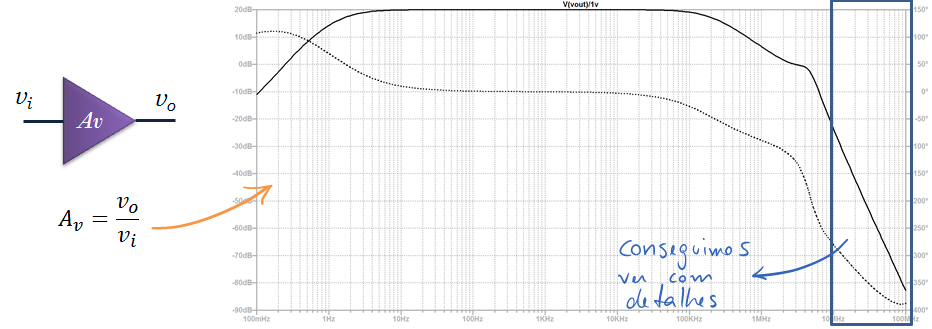
\includegraphics[width=0.6\textwidth]{imgs/diagrama2.png}
    \caption{Diagrama de Resposta em Frequência de um Ganho em dB.}
    \label{fig:ccco}
\end{figure}

É observado que continuamos a ver como o ganho do amplificador varia na faixa de 0,1 Hz a 10 MHz com uma boa resolução, como no gráfico anterior, mas na faixa de 10 MHz para cima, que antes era indistinguível, agora conseguimos ver com detalhes como o ganho se comporta. 

 Como foi mencionado antes, ao comprimir grandes números e expandir pequenos números, podemos ver num mesmo gráfico grandes variações de valores com boa resolução.
 
 Uma coisa importante para sabermos é que a conversão de uma grandeza para a representação em dB possui duas formas de ser feita, dependendo do tipo de sinal que está sendo trabalhado. Aqui iremos abordar os dois tipos.
 
 \begin{enumerate}
     \item Sinais de Potência ou Intensidade
     
     No caso de sinais de potência (W), de intensidade (sonora por exemplo), ou similares, a conversão para dB pode ser feita usando a seguinte expressão:
     
     $$
     I_{dB} = 10 \times \log_{10}\left ( \frac{I}{I_{0}} \right )
     $$
     
    \begin{center}
        Equação 11 – Conversão de sinais de potência para dB. 
    \end{center}
    
    Onde: IdB é o valor em dB; I é o valor que se deseja converter e I0 é um valor de referência.

    Como foi comentado anteriormente, a representação de uma grandeza em dB, na verdade é uma representação de uma razão entre dois números. No caso, ao convertermos um valor de intensidade sonora (por exemplo) para dB, o que estamos fazendo é converter a razão entre este número e uma base de referência para o domínio dB.

    Como exemplo, vamos usar a Intensidade Sonora, pois estamos acostumados a ler informações dessa grandeza já em dB no nosso dia-a-dia. Por definição, o valor de referência para a intensidade sonora é I0 = 10 x 10-12 W/m2.

    Com isso, se I = 10 x 10-12 W/m2 , o valor convertido para dB seria 0 dB. É interessante observar neste exemplo que toda vez que o sinal convertido tiver a mesma magnitude do sinal de referência (ou seja a razão a ser convertida é igual a um), em dB isso se equivale a 0 dB;

    Já para 1 W/m2, que é 1 trilhão de vezes maior que o sinal de referência, a conversão dá 120 dB. Esse número é interessante, pois ele é o limiar da dor, logo é um número usado como parâmetro para se definir se um determinado som em um ambiente pode causar dano à audição humana e com isso as normas de silêncio são definidas com base nele. A medição dessa grandeza é feita com um decibelímetro, como este aqui.
    
    \item Sinais de tensão, corrente, pressão sonora, etc...
    
    Agora, existe uma variação da forma de se calcular o valor de uma grandeza em dB, caso essa grandeza seja uma tensão, corrente, pressão sonora, impedância, etc. Neste caso, a expressão se torna:
    
    $$
    V_{dB}= 20 \times log_{10}\left ( \frac{V}{V_{0}} \right )
    $$
     \begin{center}
        Equação 12 – Calcular o valor de uma grandeza. 
    \end{center}
    
    Onde: VdB é o valor em dB; V é o valor que se deseja converter e V0 é um valor de referência.

    Observem que agora tem um fator de 20 multiplicando o logaritmo. Uma forma de entender o porque dessa diferença com sinais de potência é pensar na relação entre tensão e potência elétrica, por exemplo. Sabemos que a potência elétrica é proporcional ao quadrado da tensão, com isso, pensando numa escala logarítmica, 10xlog10 (V²) = 10xlog10 (V)x2 = 20xlog10 (V).

    O nível de referência obviamente depende do tipo de conversão a ser realizada. No caso de pressão sonora, para manter o exemplo anterior, o valor de referência V0 = 20 uPa. 

    Note que agora, se multiplicarmos um sinal original por 2, isso se converterá em dB como uma soma de 6 dB (e não mais 3 dB). 

    \item Como converter um sinal de dB de volta para uma base decimal
    
    A conversão reversa de dB para decimal pode ser feita se revertendo as expressões anteriores, dando origem a:
    
    $$
    I= I_{0}\times 10^{\frac{V_{dB}}{10}} 
    $$
     \begin{center}
        Equação 13
    \end{center}
    
    $$
    V= V_{0}\times 10^{\frac{V_{dB}}{20}}
    $$
    
    \begin{center}
        Equação 14
    \end{center}
 \end{enumerate}
 
 \subsection{O que é dBV, dBu e dBm?}
 Agora que já entendemos um pouco mais sobre o dB, podemos discutir sobre algumas informações que aparecem constumeiramente no ambiente de eletro-eletrônica, especialmente quando falamos no uso dessa representação em engenharia de áudio. Nesse ramo, é muito comum encontrarmos as expressões dBV, dBm e dBu, mas o que é isso?

 Bom, essas nada mais são do que formas de representação de sinais de tensão ou potência elétrica. As quais podem ser definidas como:
 \begin{itemize}
     \item dBV é uma representação de um sinal de tensão, tendo um sinal de referência de 1V;
     \item dBm é uma representação de um sinal de potência, tendo um sinal de referência de 1mW;
     \item dBu é uma representação de um sinal de tensão, tendo um sinal de referência de 0,775V. Esse por sua vez é o valor necessário para que se consuma 0 dBm (ou seja 1 mW) em uma carga de 600R;
 \end{itemize}
 
 Essas grandezas são muito comuns em equipamentos de áudio, tendo uma relação mais íntima com as origens da definição dessa representação por Graham Bell. 

 Porém, fora desse setor, costumamos usar o dB também como forma de representar diversas grandezas. Nestes casos, utilizamos mais comumente um valor de referência de 1 unidade, por exemplo, 1 V, 1 A, 1 ohm. Esses são os valores de referência que serão utilizados na conversão para dB em gráficos de resposta em frequência de simuladores de circuitos eletrônicos, por exemplo, como o LTSpice.
 
 